\subsection{\RA{}}\label{RA}
Durante il periodo precedente la \RA{} sono state apportate le modifiche necessarie a rifinire, correggere e completare il prodotto finale.
Per quanto riguarda i documenti, sono stati corretti sulla base delle indicazioni ricevute in sede di \RQ{}, quindi sono stati incrementati per aggiungere i progressi effettuati nel periodo. Secondo i risultati delle inspection effettuate in precedenza, il cui risultato è riportato nelle liste di controllo, è stata effettuata la verifica dei documenti, sottoposti infine ad approvazione da parte del \Responsabile{}.

L'avanzamento dei processi è stato verificato sulla base di quanto riportato nelle \NormeDiProgetto{}. Sono quindi state calcolate le metriche di processo e del prodotto finale e confrontate con gli obiettivi descritti in \sezione{sec:metriche_processo}.

\subsubsection{Esiti delle verifiche}
\paragraph{Indice di Gulpease}\mbox{}\\
\begin{longtable}{|c|c|c|c|c|}
	\hline \multicolumn{1}{|c|}{\textbf{Documento}} & \multicolumn{1}{c|}{\textbf{Risultato}} & \multicolumn{1}{c|}{\textbf{Accettazione}} & \multicolumn{1}{c|}{\textbf{Ottimalità}} & \multicolumn{1}{c|}{\textbf{Esito}}\\
	\hline 
	\endfirsthead
	
	\hline \multicolumn{1}{|c|}{\textbf{Documento}} & \multicolumn{1}{c|}{\textbf{Risultato}} & \multicolumn{1}{c|}{\textbf{Accettazione}} & \multicolumn{1}{c|}{\textbf{Ottimalità}} & \multicolumn{1}{c|}{\textbf{Esito}}\\
	\hline 
	\endhead
	
	\hline \multicolumn{5}{|r|}{\ToBeContinued} \\ 
	\hline
	\endfoot
	
	\endlastfoot
	
	\hline \NormeDiProgetto{} & 80 & 40-100 & 50-100 & Superato\\
	\hline \PianoDiProgetto{} & 80 & 40-100 & 50-100 & Superato \\
	\hline \PianoDiQualifica{} & 82 & 40-100 & 50-100 & Superato \\
	\hline \AnalisiDeiRequisiti{} & 92 & 40-100 & 50-100 & Superato \\
	\hline \Glossario{} & 65 & 40-100 & 50-100 & Superato \\
	\hline \SpecificaTecnica{} & 85 & 40-100 & 50-100 & Superato\\
	\hline \DefinizioneDiProdotto{} & 78 & 40-100 & 50-100 & Superato\\
	\hline Demo User manual & 8.3 & 6-12 & 6-10 & Superato\\
	\hline Framework User manual & 7.9 & 6-12 & 6-10 & Superato\\
	\hline VerbaleInterno 18\_06\_2017 & 87 & 40-100 & 50-100 & Superato \\
	\hline VerbaleEsterno 11\_06\_2017 & 70 & 40-100 & 50-100 & Superato \\
	\hline VerbaleInterno 25\_04\_2017 & 75 & 40-100 & 50-100 & Superato \\
	\hline VerbaleInterno 10\_04\_2017 & 93 & 40-100 & 50-100 & Superato \\
	\hline VerbaleInterno 29\_03\_2017 & 85 & 40-100 & 50-100 & Superato \\
	\hline VerbaleEsterno 22\_03\_2017 & 68 & 40-100 & 50-100 & Superato \\
	\hline VerbaleInterno 2\_03\_2017 & 73 & 40-100 & 50-100 & Superato \\
	\hline VerbaleInterno 23\_02\_2017 & 83 & 40-100 & 50-100 & Superato \\
	\hline VerbaleInterno 30\_01\_2017 & 85 & 40-100 & 50-100 & Superato \\
	\hline VerbaleInterno 30\_12\_2016 & 84 & 40-100 & 50-100 & Superato \\
	\hline VerbaleEsterno 23\_12\_2016 & 75 & 40-100 & 50-100 & Superato \\
	\hline VerbaleInterno 22\_12\_2016 & 85 & 40-100 & 50-100 & Superato \\
	\hline VerbaleInterno 16\_12\_2016 & 83 & 40-100 & 50-100 & Superato \\
	\hline VerbaleInterno 9\_12\_2016 & 80 & 40-100 & 50-100 & Superato \\
	\hline VerbaleEsterno 8\_12\_2016 & 79 & 40-100 & 50-100 & Superato \\
	\hline
	\caption{Valori indice di Gulpease/Gunnig Fog - \RA{}}
\end{longtable}


\paragraph{Fallimento dei test}\mbox{}\\
La percentuale di test falliti sulla compilazione dei documenti e del codice ottenuta è del 7\%, un valore che ricade nel range di accettazione di questa metrica secondo quanto imposto da questo documento. \\
Il fallimento rilevato deriva principalmente dalla riorganizzazione dei contenuti nel codice sorgente e dal processo di integrazione a cui è stata sottoposta la \DemoName{}, la quale ora si attiene molto più allo stile del framework, utilizzandolo in tutte le sue parti.\\
A seguire il grafico della tendenza di successo e fallimento dei test eseguiti:
\begin{figure}[H]
	\centering
	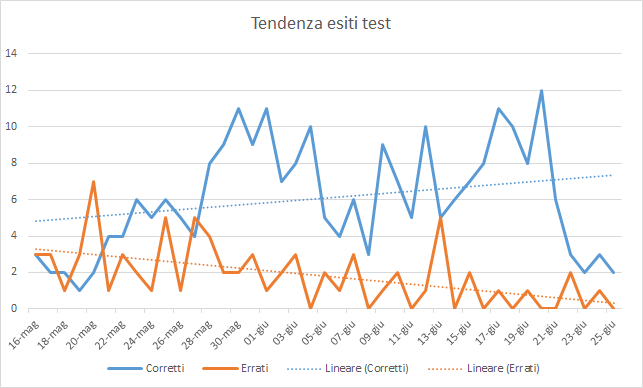
\includegraphics[width=15cm]{./test.png}
	\caption{Tendenza esito test eseguiti}
\end{figure}

\paragraph{Metriche di progettazione e di codifica}\mbox{}\\
Vengono ora presentati i risultati ottenuti dalle misurazioni relativamente alle metriche di progettazione e di codifica:
\begin{longtable}{|m{5cm}|c|c|c|c|}
	\hline \multicolumn{1}{|c|}{\textbf{Metrica}} & \multicolumn{1}{c|}{\textbf{Risultato}} & \multicolumn{1}{c|}{\textbf{Accettazione}} & \multicolumn{1}{c|}{\textbf{Ottimalità}} & \multicolumn{1}{c|}{\textbf{Esito}}\\
	\hline 
	\endfirsthead
	
	\hline \multicolumn{1}{|c|}{\textbf{Metrica}} & \multicolumn{1}{c|}{\textbf{Risultato}} & \multicolumn{1}{c|}{\textbf{Accettazione}} & \multicolumn{1}{c|}{\textbf{Ottimalità}} & \multicolumn{1}{c|}{\textbf{Esito}}\\
	\hline 
	\endhead
	
	\hline \multicolumn{5}{|r|}{\ToBeContinued} \\ 
	\hline
	\endfoot
	
	\endlastfoot
	
	\hline Fan-in medio & 1.5 & >=0 & >=2 & Superato \\
	\hline Fan-out medio & 2.5 & 0-5 & 0-1 & Superato \\
	\hline Complessità ciclomatica & 2.4 & 1-15 & 1-10 & Superato \\
	\hline Parametri per metodo & 0.5 & 0-7 & 0-4 & Superato \\
	\hline Halstead: difficoltà & 10 & 0-25 & 0-15 & Superato \\
	\hline Halstead: sforzo complessivo & 415 & 0-400 & 0-300 & Non superato\\
	\hline Halstead: volume & 657 & 20-1500 & 20-1000 & Superato \\
	\hline Core size & 18 & 0-50 & 0-40 & Superato \\
	\hline Indice di manutenibilità & 133 & 90-171 & 120-171 & Superato \\
	\hline Code coverage & 65 & 40-100 & 60-100 & Superato \\
	\hline Branch coverage & 70 & 70-100 & 80-100 & Superato \\
	\hline Function coverage & 65 & 70-100 & 80-100 & Non superato \\
	\hline Test di unità eseguiti & 85 & 85-100 & 100 & Superato \\
	\hline Test di integrazione eseguiti & 68 & 60-100 & 70-100 & Superato \\
	\hline Test di sistema eseguiti & 70 & 70-100 & 80-100 & Superato \\
	\hline Test superati & 90 & 85-100 & 100 & Superato \\
	\hline
	\caption{Metriche di processo - \RA{}}
\end{longtable}

\paragraph{Metriche di prodotto}\mbox{}\\
\begin{longtable}{|m{5cm}|c|c|c|c|}
	\hline \multicolumn{1}{|c|}{\textbf{Metrica}} & \multicolumn{1}{c|}{\textbf{Risultato}} & \multicolumn{1}{c|}{\textbf{Accettazione}} & \multicolumn{1}{c|}{\textbf{Ottimalità}} & \multicolumn{1}{c|}{\textbf{Esito}}\\
	\hline 
	\endfirsthead
	
	\hline \multicolumn{1}{|c|}{\textbf{Metrica}} & \multicolumn{1}{c|}{\textbf{Risultato}} & \multicolumn{1}{c|}{\textbf{Accettazione}} & \multicolumn{1}{c|}{\textbf{Ottimalità}} & \multicolumn{1}{c|}{\textbf{Esito}}\\
	\hline 
	\endhead
	
	\hline \multicolumn{5}{|r|}{\ToBeContinued} \\ 
	\hline
	\endfoot
	
	\endlastfoot
	
	\hline Functional size measurement & 75 & 80-100 & 100 & Non superato \\
	\hline Accuratezza rispetto alle attese & 92 & 90-100 & 100 & Superato \\
	\hline Fallimento dei test & 7 & 0-15 & 0 & Superato \\
	\hline Parametri per metodo & 0.5 & 0-7 & 0-4 & Superato \\
	\hline
	\caption{Metriche di prodotto - \RA{}}
\end{longtable}
